\question
Представьте, что вы путешествуете по острову "Итмолэнд", который представляет собой большой прямоугольник размером 10*6 км. На этом острове тропинки идут строго параллельно берегам. На каждой развилке вы можете выбрать только 2 направления: либо вправо, либо вверх. Вам нужно добраться из точки A, расположенной в левом нижнем углу острова, в точку B, которая находится в правом верхнем углу.

Какое количество различных маршрутов существует для того, чтобы успешно добраться от точки A до точки B?

\begin{minipage}[h]{0.45\linewidth}
\center{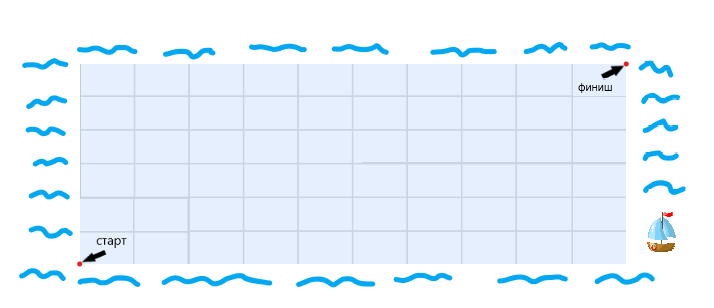
\includegraphics[width=0.7\textwidth]{pic/12.png} }
\end{minipage}

---------------

Автор -- Александр Лазарев
